\chapter{Saisie Rapide}
\section*{}
La recopie incrémentée permet un gain de temps considérable, en vous évitant de répéter maintes fois les mêmes opérations. Pour ce faire, placez le pointeur sur l’extrémité inférieure droite de la sélection, cliquez sans 
relâcher ensuite dirigez le pointeur jusqu'a la cellule de destination.
\section{Succession de Repetition} 
\begin{center}  
	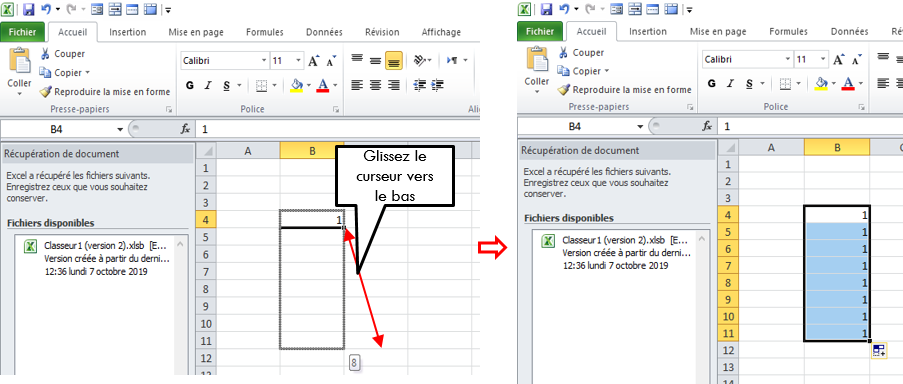
\includegraphics[scale=0.2,width=0.9 \linewidth]{img/saisi_rapide1} 
	\captionof{figure}{Bordure des cellules} 
\end{center}
\section{Suite Inscrementée}
\begin{center}  
	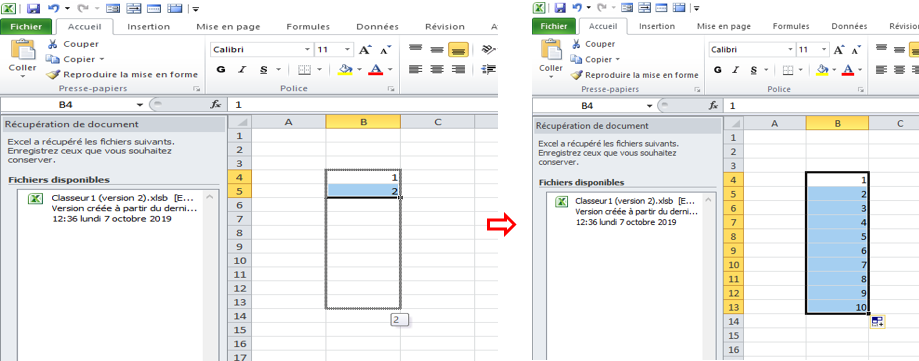
\includegraphics[scale=0.2,width= \linewidth]{img/saisi_rapide2}
	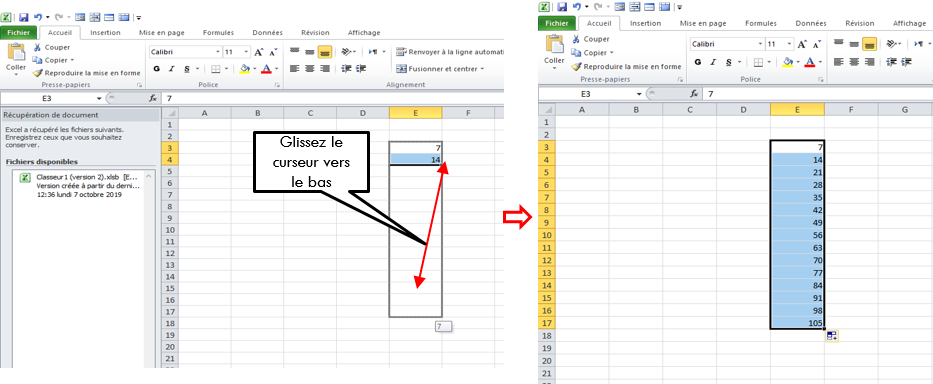
\includegraphics[scale=0.2,width= \linewidth]{img/saisi_rapide3}
	\captionof{figure}{Aligment text} 
\end{center}

\section{Suite Inscrementée  d'une liste personnalisée }
\begin{center}  
	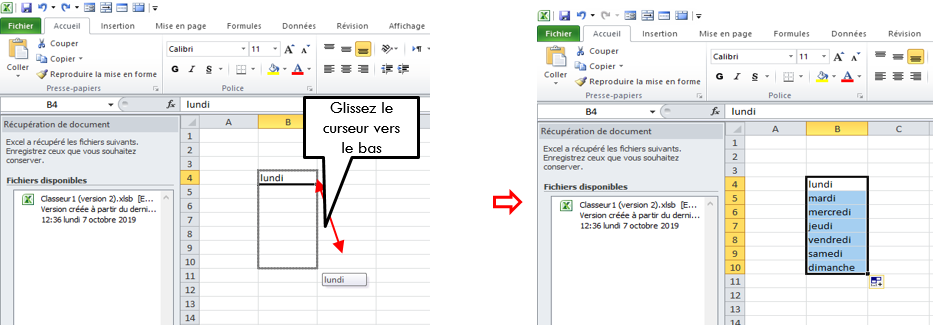
\includegraphics[scale=0.2,width= \linewidth]{img/saisi_rapide4}
	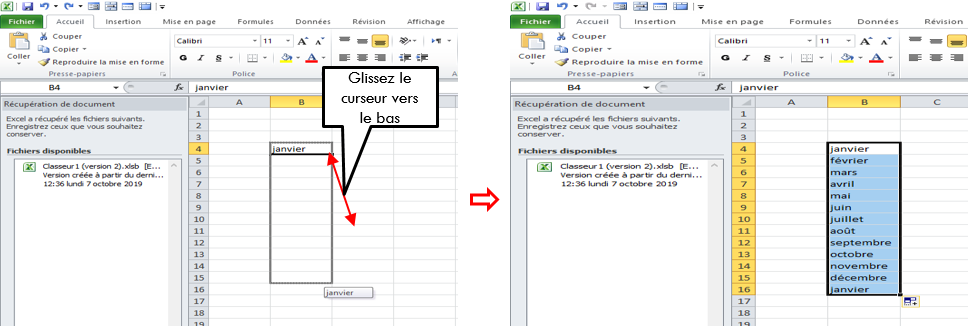
\includegraphics[scale=0.2,width= \linewidth]{img/saisi_rapide5}
	\captionof{figure}{Aligment text} 
\end{center}

\section{Liste personnalisée }
\begin{center}  
	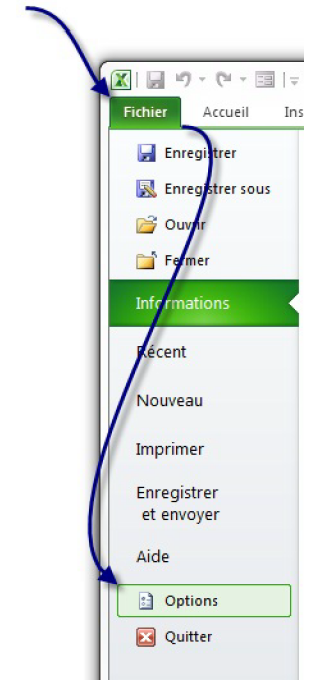
\includegraphics[scale=0.2,width=0.2 \linewidth]{img/saisi_rapide6}
	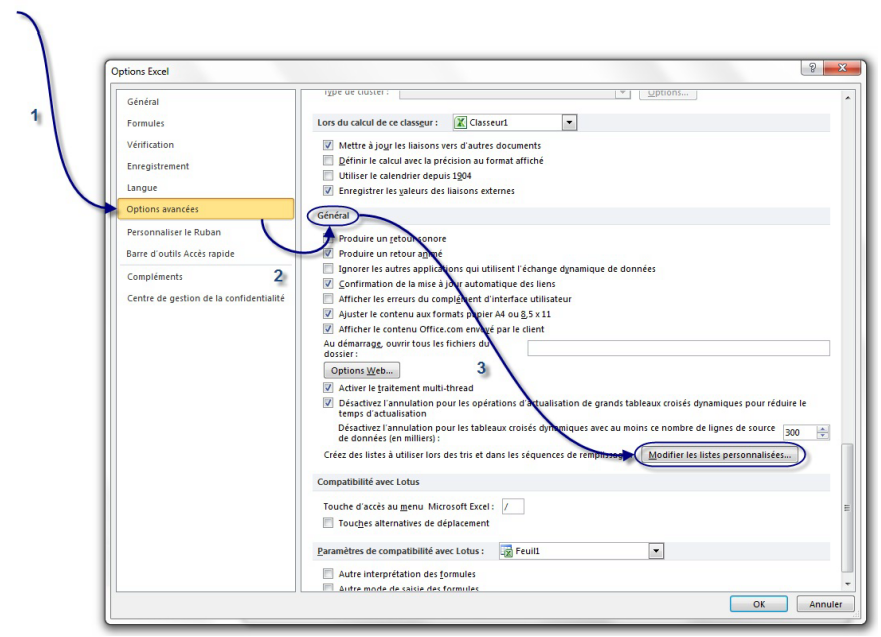
\includegraphics[scale=0.2,width= \linewidth]{img/saisi_rapide7}
	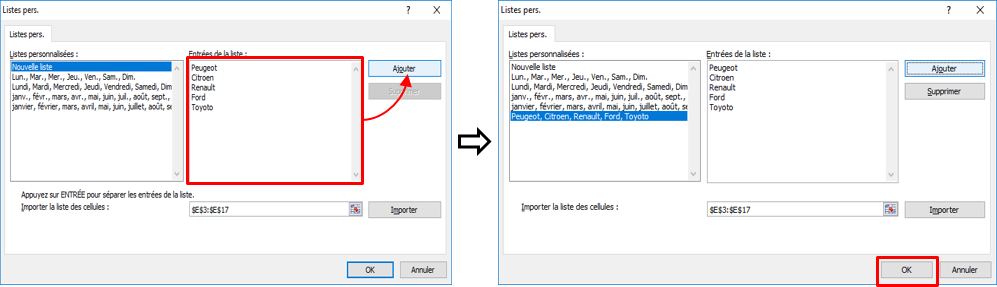
\includegraphics[scale=0.2,width= \linewidth]{img/saisi_rapide8}
	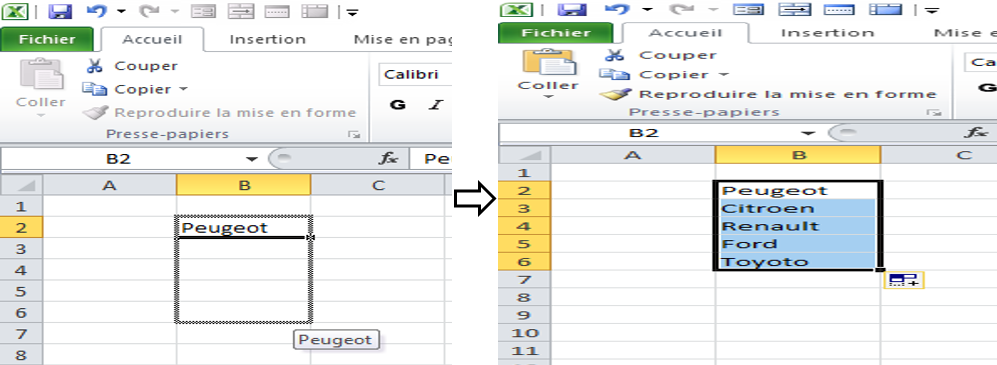
\includegraphics[scale=0.2,width= \linewidth]{img/saisi_rapide9} 
\end{center}

\section{Série d'Exercices}
\begin{exercice}\label{ex4}
	Consignes 
	\begin{enumerate}		
		\item  Saisir  le tableau suivant.
	\end{enumerate}
\end{exercice} 
\begin{figure}[H]  
	\centering
	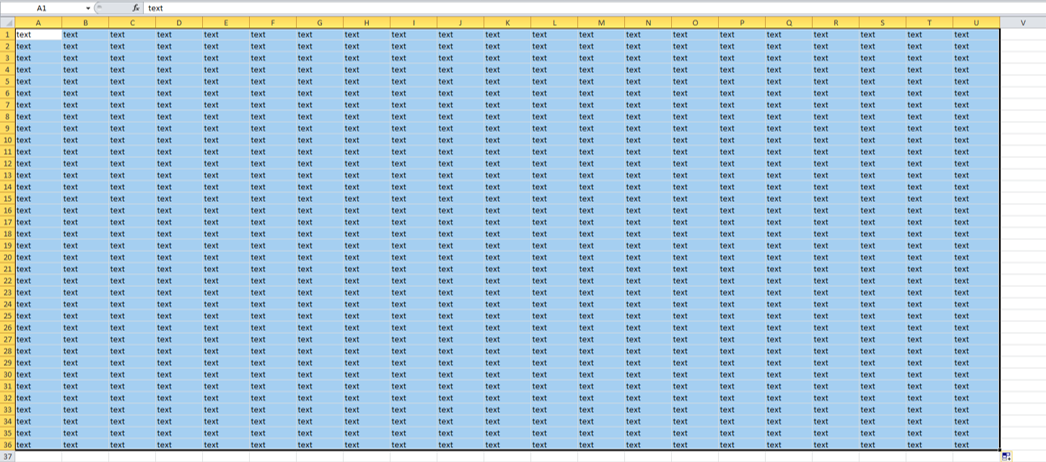
\includegraphics[scale=0.2,width= \linewidth]{img/ex04} 
	\captionof{figure}{Exercice \ref{ex4}} 
\end{figure} 

\begin{exercice}\label{ex5}
	Consignes 
	\begin{enumerate}		
		\item  Saisir  le tableau suivant		
	\end{enumerate}
\end{exercice}  
\begin{figure} [H]  
	\centering
	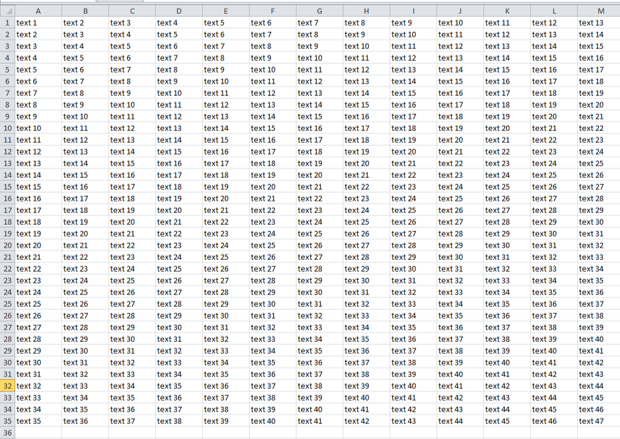
\includegraphics[scale=0.2,width= \linewidth]{img/ex05} 
	\captionof{figure}{Exercice \ref{ex5}} 
\end{figure}
\begin{exercice}\label{ex6}
	Consignes 
	\begin{enumerate}		
		\item  A l'aide du saisie rapide Saisiez le tableau suivant.  				
		\item  Mettre la mise en forme le tableau: largeur colonne:4, centré le contenue du tableau, taille de police:11, police: Calibri.				
		\item  Saisir le titre et le centré horizontalement et veriticalement, police:18, police: Calibri, style:Gras.
	\end{enumerate}	
\end{exercice}
\begin{figure}[H]
	\centering
	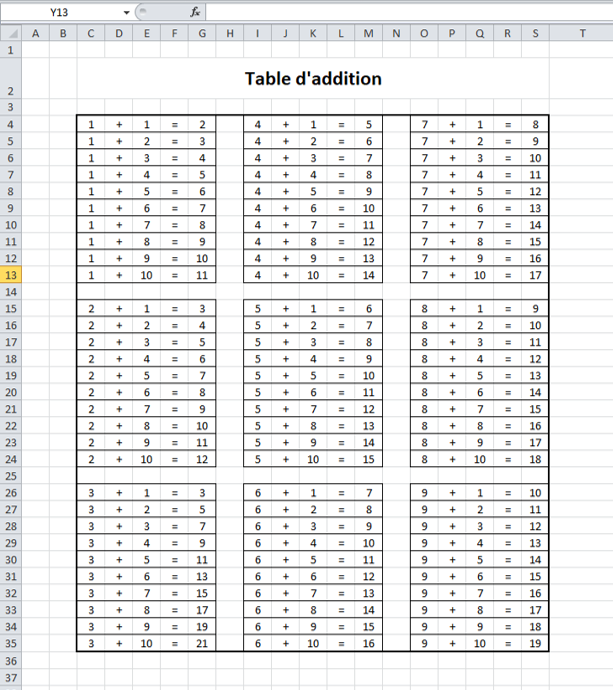
\includegraphics[scale=0.2,width=0.7 \linewidth]{img/ex06}
	\captionof{figure}{Exercice \ref{ex6}} 
\end{figure}

\begin{exercice}\label{ex7}
	Consignes 
	\begin{enumerate}	
		\item Créer une liste personnalisée : \textbf{a,b,c,d,e,f,g,h,i,j,k,l,m,n,o,p,q,r,s,t,u,v,w,x,y,z}
		\item Créer une liste personnalisée : \textbf{z,y,x,w,v,u,t,s,r,q,p,o,n,m,l,k,j,i,h,g,f,e,d,c,b,a}		
		\item  A l'aide du saisie rapide realiser le tableau suivant.  				
		\item  Mettre la mise en forme le tableau:bordure, trame, largeur colonne:4, centré le contenue du tableau, taille de police:11, police: Calibri.
	\end{enumerate}	
\end{exercice}
\begin{figure}[H]
	\centering
	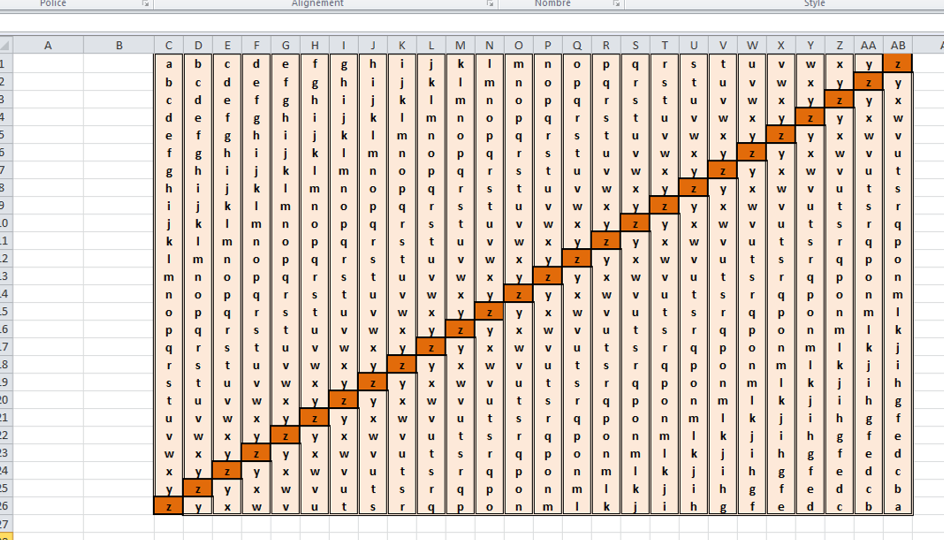
\includegraphics[scale=0.2,width=0.7 \linewidth]{img/ex07}
	\captionof{figure}{Exercice \ref{ex7}} 
\end{figure}
